% -*- fill-column: 80; comment-column: 50; -*-
%--------- adjust textmate window until this just fits --------------------------

\documentclass{article}

% \VignetteIndexEntry{Introduction to oce}
% \VignetteDepends{oce}
% \VignetteKeyword{oceanography}

\usepackage{url}
\usepackage{fullpage}
\usepackage{boxedminipage}
\usepackage{hyperref}
\usepackage{makeidx}
\usepackage{titlesec}
\makeindex

\parskip=1.5ex plus 1.5ex minus 1.25ex

\titleformat{\section}[block]{\normalfont\large\bfseries}{\thesection}{1em}{}
\titlespacing{\section}{0em}{2em plus 3em minus 0.5em}{0.15em plus 0.15em minus 0.125em}
\titleformat{\subsection}[block]{\normalfont\large\itshape}{\thesubsection}{1em}{}
\titlespacing{\subsection}{0em}{1em plus 2em minus 0.5em}{-0.15em plus 0.15em minus 0.125em}

\newcommand{\workedexercise}[2]{
	\vspace{2ex plus 2ex minus 1ex}
	\begin{boxedminipage}[c]{0.95\linewidth}
		{\textbf{Exercise #1}.\hspace{1em}#2}
	\end{boxedminipage}
	\vspace{2ex plus 2ex minus 1ex}
}
\newcommand{\workedanswer}[2]{
\goodbreak
\vskip 1.5ex plus 0.5ex minus 0.5ex
\noindent\textbf{Exercise #1 -- #2.}
}


\usepackage{/Library/Frameworks/R.framework/Resources/share/texmf/Sweave}
\begin{document}

\title{The OCE package}
\author{Dan E. Kelley}
\maketitle


\begin{abstract}

The \verb@oce@ package makes it easy to read, summarize and plot data from a
variety of Oceanographic instruments, isolating the researcher from the quirky
data formats that are common in this field. It also provides functions for
working with basic seawater properties such as the equation of state, and with
derived quantities such as the buoyancy frequency.  Although simple enough to be
used in a teaching context, \verb@oce@ is powerful enough for a research
setting.  These things are illustrated here with practical examples.

\end{abstract}

\section{Introduction}

Oceanographers must deal with measurements made by a wide variety of
instruments, a task that is complicated by the delight instrument manufacturers
seem to take in inventing new data formats. The manufacturers often provide
software for scanning the data files and producing some standard plots, but this
is of limited use to researchers who work with several instrument types at the
same time, and who need to carry the analysis beyond the first step.

The need to scan diverse data files was one motivation for the creation of
\verb@oce@, but an equal goal was to make it easy to work with the data once
they are in the system.  This was accomplished partly by the provision of
functions to work with the data, and partly by developing a uniform object
design that lets users reach inside without guesswork\footnote{Each \texttt{oce}
object is a list containing three elements: (a) \texttt{data}, a list or a data
frame containing the actual data, for a CTD object, this will contain pressure,
temperature, etc., (b) \texttt{metadata}, a list containing data such things as
file headers, the location of a CTD cast, etc., and (c) \texttt{processing.log},
a list that documents how the file was created (often by a \texttt{read} or
\texttt{as} method) and how it was changed thereafter (e.g. by decimating a CTD
cast).}, and partly by adhering to a policy of adding features according to the
priorities of practical research. The net result is that \verb@oce@ is a fairly
comfortable tool today, and one that should to remain so as it grows.


\section{Calculations of seawater properties}

\index{calculation!seawater properties}
\index{seawater properties, calculations of}

The \verb@oce@ package provides many functions for dealing with seawater
properties. Probably the most used is \verb@sw.rho(S,t,p)@, which computes
seawater density $\rho$ as a function of salinity $S$ (PSU), in-situ temperature
$t$ ($^\circ$C \dots\/ note the use of lower-case in this and related functions,
to avoid confusion with \verb@T@, an abbreviation used sometimes in R programs)
and pressure $p$ (decibar). The result is a number in the order of
$1000$kg/m$^3$.  For many purposes, Oceanographers prefer to use the density
anomaly $\sigma=\rho-1000$kg/m$^3$, provided with \verb@sw.sigma(S,t,p)@, or its
adiabatic cousin $\sigma_\theta$, provided with \verb@sw.sigma.theta(S,t,p)@.

Note that the names of functions relating to seawater material properties start
with ``\verb@sw.@''; future versions of \verb@oce@ may add similarly named
functions for the properties of air, sediment, organisms, etc.

The \verb@sw.@ functions can also take a \verb@ctd@ object instead of the
\verb@(S, t, p)@ arguments.

\looseness=1
\index{dynamic height}
Most of the functions use the UNESCO formulations of seawater properties, but new formulations
may be added as they come into use in the literature.
A partial list of seawater functions is as follows:
\verb@sw.dynamic.height@ (dynamic height),
\verb@sw.N2@ (buoyancy freqency),
\verb@sw.S.C.T.p@ (salinity $S$ from $C$, $T$ and $p$),
\verb@sw.S.T.rho@ ($S$ from $T$ and $\rho$),
\verb@sw.T.S.rho@ ($T$ from $S$ and $\rho$),
\verb@sw.T.freeze@ (freezing temperature),
\verb@sw.alpha@ (thermal expansion coefficient $\alpha=-\rho_0^{-1}\partial\rho/\partial T$),
\verb@sw.beta@ (haline compression coefficient $\beta=\rho_0^{-1}\partial\rho/\partial S$),
\verb@sw.alpha.over.beta@ ($\alpha/\beta$),
\verb@sw.conductivity@ (conductivity from $S$, $T$ and $p$),
\verb@sw.depth@ (depth from $p$ and latitude),
\verb@sw.lapse.rate@ (adiabatic lapse rate),
\verb@sw.rho@ (density $\rho$ from $S$, $T$ and $p$),
\verb@sw.sigma@ ($\rho-1000$\,kg/m$^3$),
\verb@sw.sigma.t@ ($\sigma$ with $p$ set to zero and temperature unaltered),
\verb@sw.sigma.theta@ ($\sigma$ with $p$ set to zero and temperature altered adiabatically),
\verb@sw.sound.speed@ (speed of sound in m/s),
\verb@sw.specific.heat@ (specific heat in J/kg/$^\circ$C),
\verb@sw.spice@ (a quantity used in double-diffusive research),
\verb@sw.theta@ (potential temperature in $^\circ$C),
and
\verb@sw.viscosity@ (viscosity).
Details and examples are, of course, provided in the documentation of these functions.


\workedexercise{1}{(a) What is the density of a seawater parcel at pressure
$100$dbar, with salinity $34$PSU and temperature $10^\circ$C?
(b) What temperature would the parcel have if raised adiabatically to the surface?
(c) What density would it have if raised adiabatically to the surface?
(d) What density would it have if lowered about 100m, increasing the pressure to $200$dbar?
(e) Draw a blank TS diagram with $S$ from $30$ to $40$PSU and $T$ from $-2$ to $20^\circ C$.  (Answers are provided at the end of this document.)
}


\section{CTD data}
\subsection{Example with pre-trimmed data}

\index{data!ctd profile \verb@ctd@}

To get you started with CTD data, \verb@oce@ provides a sample data set that has
been trimmed to just the downcast portion of the sampling.  (See the next
section to learn how to do this trimming.).  The commands
\begin{Schunk}
\begin{Sinput}
> library(oce)
> data(ctd)
> plot(ctd)
\end{Sinput}
\end{Schunk}
produce Figure~\ref{fig:ctd}. You may also get a summary of the data with
\begin{Schunk}
\begin{Sinput}
> summary(ctd)
\end{Sinput}
\end{Schunk}

The object used to hold CTD data stores not just the data, but also the raw
header sequence, and whatever has been discovered about the dataset by parsing
the header; use
\begin{Schunk}
\begin{Sinput}
> names(ctd)
\end{Sinput}
\end{Schunk}
to learn about these metadata, and use
\begin{Schunk}
\begin{Sinput}
> names(ctd$data)
\end{Sinput}
\end{Schunk}
to find out what sensors were attached to the instrument, thus providing data columns.

As noted above, the seawater-property functions (whose names begin with
\verb@sw.@) can take a \verb@ctd@ object instead of the individual arguments
\verb@S@, \verb@t@, and \verb@p@.

It is possible to plot the components of a \verb@ctd@ object individually,
either by accessing the data directly (see the WOCE section, below, for an
example) or by using more specialized functions such as
\verb@plot.TS@ and \verb@plot.profile@.
\begin{figure}
\begin{center}
\setkeys{Gin}{width=.8\textwidth}
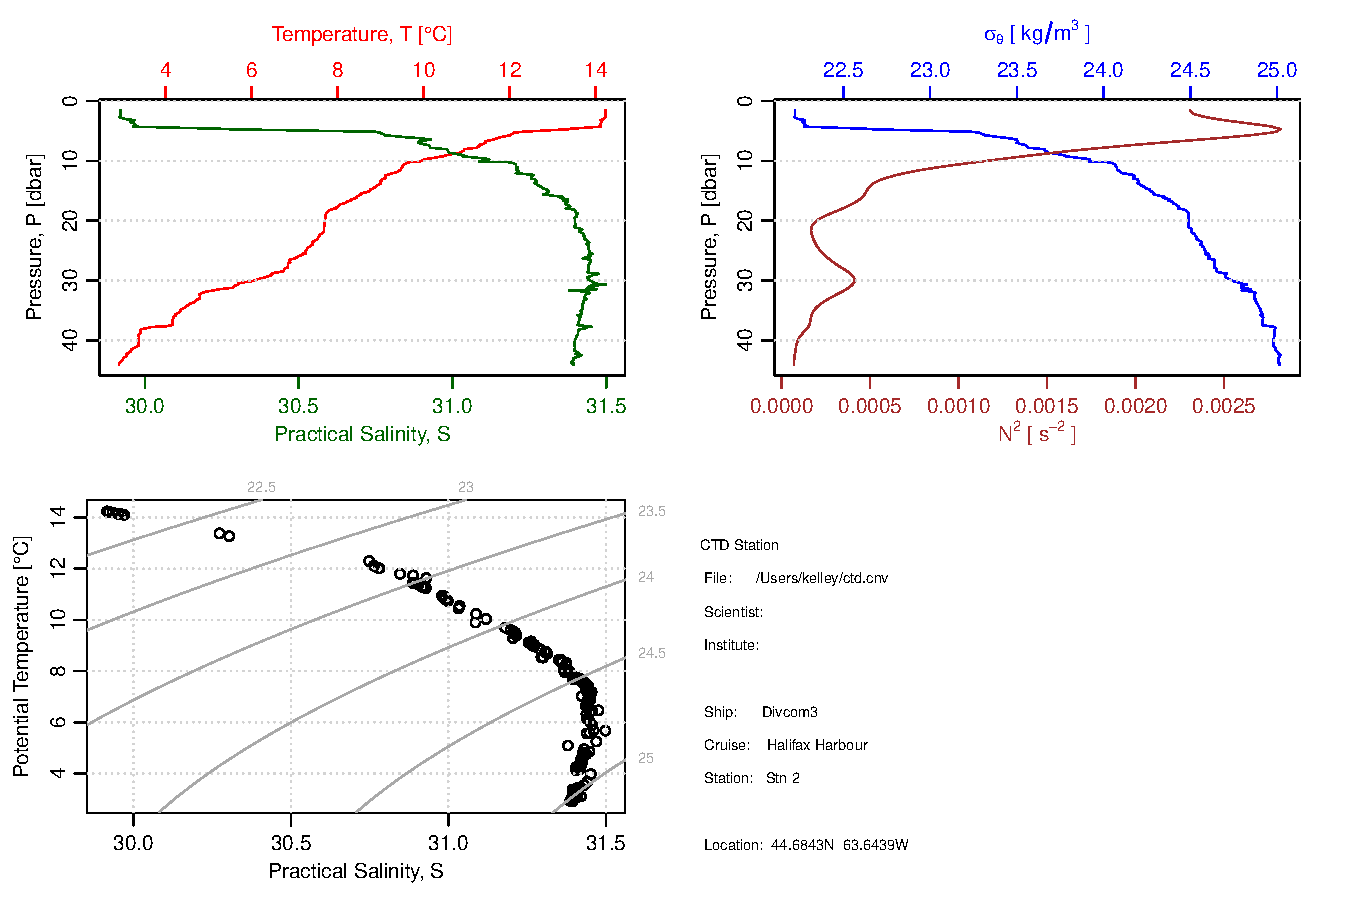
\includegraphics{oce-ctdfig}
\end{center}
\caption{Overview graph of the sample CTD dataset \texttt{ctd}, acquired during
the St Lawrence Estuary Internal Wave Experiment.  (This dataset has been
trimmed to just the downcast; see the text and Figure~\ref{fig:ctdraw} for more
on trimming.)}
\label{fig:ctd}
\end{figure}

\workedexercise{2}{Plot a profile of $\sigma_\theta$ and $N^2$, for just the data in the pycnocline.}

\subsection{Example with raw data}

Practicing Oceanographers may be wondering how the CTD cast used in the
preceding section was trimmed of equilibration-phase and upcast-phase data. Data
from these sections are spurious and must be trimmed as a first step in
processing. For example, consider the following code.
\begin{Schunk}
\begin{Sinput}
> data(ctd.raw)
> plot.ctd.scan(ctd.raw)
\end{Sinput}
\end{Schunk}
\begin{figure}
\begin{center}
\setkeys{Gin}{width=0.55\textwidth}
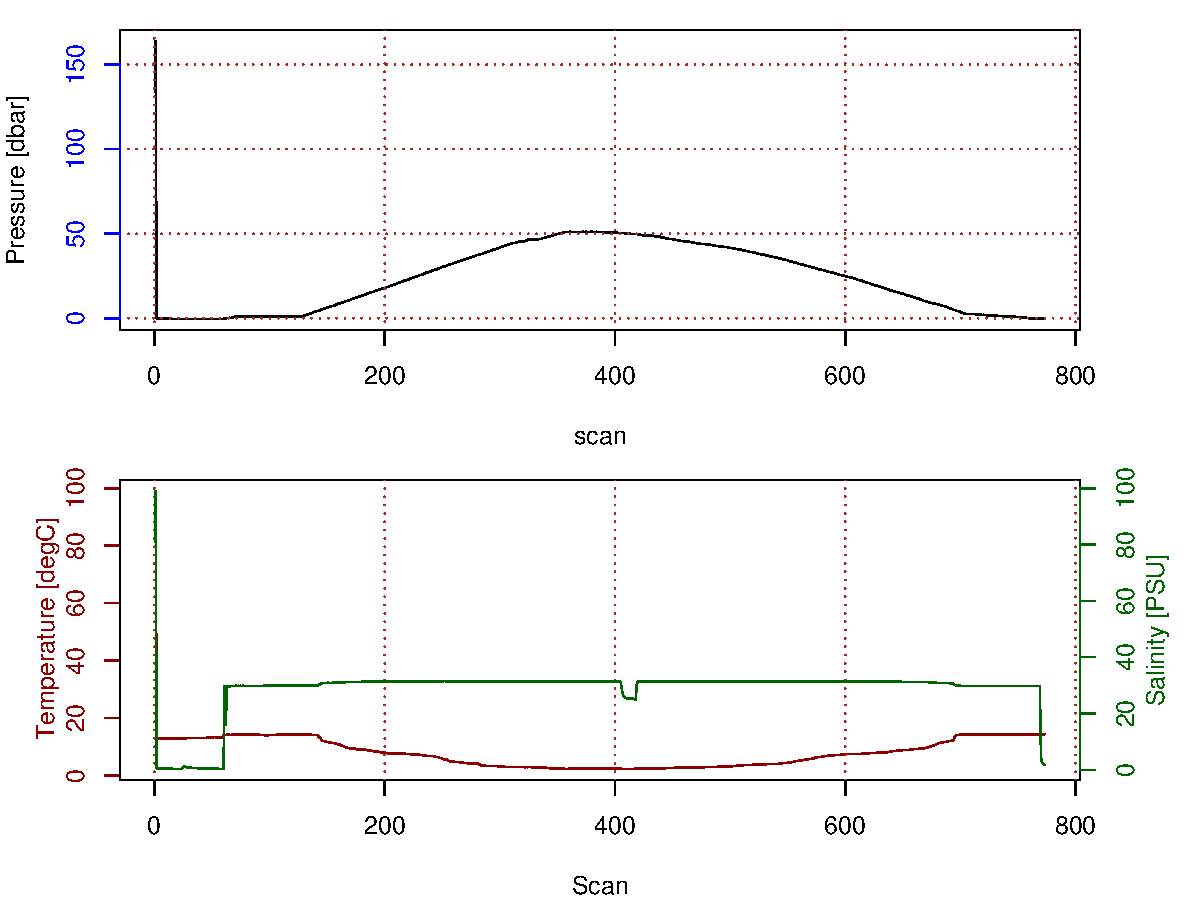
\includegraphics{oce-ctdrawfig}
\end{center}
\caption{Scanwise plot of the \texttt{ctd.raw} sample data set.  Note the wild
spike at the start, the equilibration phase before the downcast, and the
spurious freshening signal near the start of the upcast.  See the text for a
discussion of how inspection of such graphs can help in trimming CTD data.}
\label{fig:ctdraw}
\end{figure}

\noindent This produces a two-panel plot (Figure~\ref{fig:ctdraw}) of the data
as a time-series, revealing not just the (useful) downcast, but also the
subsequent upcast sequence.  The x-axis in this plot is the scan number, which
is a convenient index for extraction of the downcast portion of the profile by
an essentially manual method, e.g. proceeding with a sequence of commands such
as
\begin{Schunk}
\begin{Sinput}
> plot.ctd.scan(ctd.trim(ctd.raw, "scan", c(140, 250)))
> plot.ctd.scan(ctd.trim(ctd.raw, "scan", c(150, 250)))
\end{Sinput}
\end{Schunk}
This is the ``gold standard'' method, which is recommended for detailed
work. However, for quick work, you may find that the automatic downcast
detection scheme works adequately, e.g.
\begin{Schunk}
\begin{Sinput}
> ctd.trimmed <- ctd.trim(ctd.raw)
\end{Sinput}
\end{Schunk}

It should be noted that \verb@ctd.trim@ inserts entries into the object's log
file, so that you (or anyone else with whom you share the object) will be able to
see the details of how the trimming was done.

\index{reading!ctd profile}

Once the profile has been trimmed, you may wish to use \texttt{ctd.decimate()}
to smooth the data and interpolate the smoothed results to uniformly-spaced
pressure values. For example, a quick examination of a file might be done by the
following:
\begin{Schunk}
\begin{Sinput}
> plot(ctd.decimate(ctd.trim(read.ctd("stn123.cnv"))))
\end{Sinput}
\end{Schunk}

\subsection{Example with WOCE archive data}

The package has a harder time scanning the headers of data files in the WOCE
archive format than it does in the Seabird format illustrated in the previous
examples. This is mainly because front-line researchers tend to work in the
Seabird format, and partly because the WOCE format is odd. For example, the
first line of a WOCE file is of the form \texttt{CTD,20060609WHPOSIODAM}.  Only
the first part of this is easy to scan. To the left of the comma is the string
\texttt{CTD}, which seems straightforward, except that in some cases it is
written \texttt{CTDO}. After the comma is found the file date (yyyymmdd), and
that is easy to parse. But then things get tricky.  The next sequence is a
string of characters that indicate the division of the institute (WHPO), the
institute itself (SIO), and the name of the investigator (DAM). The problem is
that no dividers separate these items, and that there are no standards for the
item lengths. The approach to \verb@oce@ development is to tackle easy and
important problemss before complicated special cases, and so no attempt has been
made to parse this part of the header. Of course, R provides access to object
constituents, so that a human working with this file could easily do e.g.
\begin{Schunk}
\begin{Sinput}
> x <- read.ctd("nnsa_00934_00001_ct1.csv", type = "WOCE")
> x$metadata$institute <- "SIO"
> x$metadata$scientist <- "DAM"
\end{Sinput}
\end{Schunk}

For a real-world example (with warts!), visit
\url{http://cchdo.ucsd.edu/data_access?ExpoCode=58JH199410} and download the zip
file containing the Arctic section called ``CARINA'', measured in 1994. Expand
the zip file, enter the directory, and run the code below.
\begin{Schunk}
\begin{Sinput}
> library(oce)
> files <- system("ls *.csv", intern = TRUE)
> for (i in 1:length(files)) {
+     cat(files[i], "\n")
+     x <- read.ctd(files[i])
+     if (i == 1) {
+         plot.TS(x, xlim = c(31, 35.5), ylim = c(-1, 10), type = "l", 
+             col = "red")
+     }
+     else {
+         lines(x$data$salinity, x$data$temperature, col = "red")
+     }
+ }
\end{Sinput}
\end{Schunk}

What you'll see is an overall $T-S$ diagram for the entire dataset. It may take
a while, since the dataset contains over 90,000 observations. You may note that,
even though this is an official, quality-controlled dataset, it is not without
problems. The graph that is produced by this code has several spurious lines
oriented horizontally (indicating spurious salinity) and vertically (indicating
spurious temperature). One way to find such values is to put the lines
\begin{Schunk}
\begin{Sinput}
> print(range(x$data$temperature))
> print(range(x$data$salinity))
\end{Sinput}
\end{Schunk}
after the \verb@read.ctd()@ command. One thing you'll find is that station 987
has a minimum salinity range of 0.0009 to 987. These values are clearly in
error, as are the temperatures at this spot in the file. (It is perhaps
revealing that the spurious salinity is equal to the station number.) Indeed, at
this spot in the file it can be seen that the pressure jumps from 1342 to 0, and
then starts increasing again; the file contains two profiles, or the same
profile twice. This is not the only flaw that is revealed by the graph, and by
\verb@range@ commands; a generous user would spend a week tracking down such
issues, and would then contact the data provider (or the chief scientist of the
field work) with specific suggestions for correcting the files. The point here
is to highlight how this package can be used with real-world data.

\subsection{Section plots}
The commands
\begin{Schunk}
\begin{Sinput}
> data(section)
> data(coastline.hal)
> plot(section, coastline = coastline.hal)
\end{Sinput}
\end{Schunk}
will plot a summary diagram (Figure~\ref{fig:section}) containing sections of
$T$, $S$, and $\sigma_\theta$, along with a chart indicating station
locations. In addition to such overview diagrams, \verb@plot@ can also create
individual plots of individual properties.

\workedexercise{3}{Draw a TS diagram for the section data, colour-coded by station}

\begin{figure}
\begin{center}
\setkeys{Gin}{width=1\textwidth}
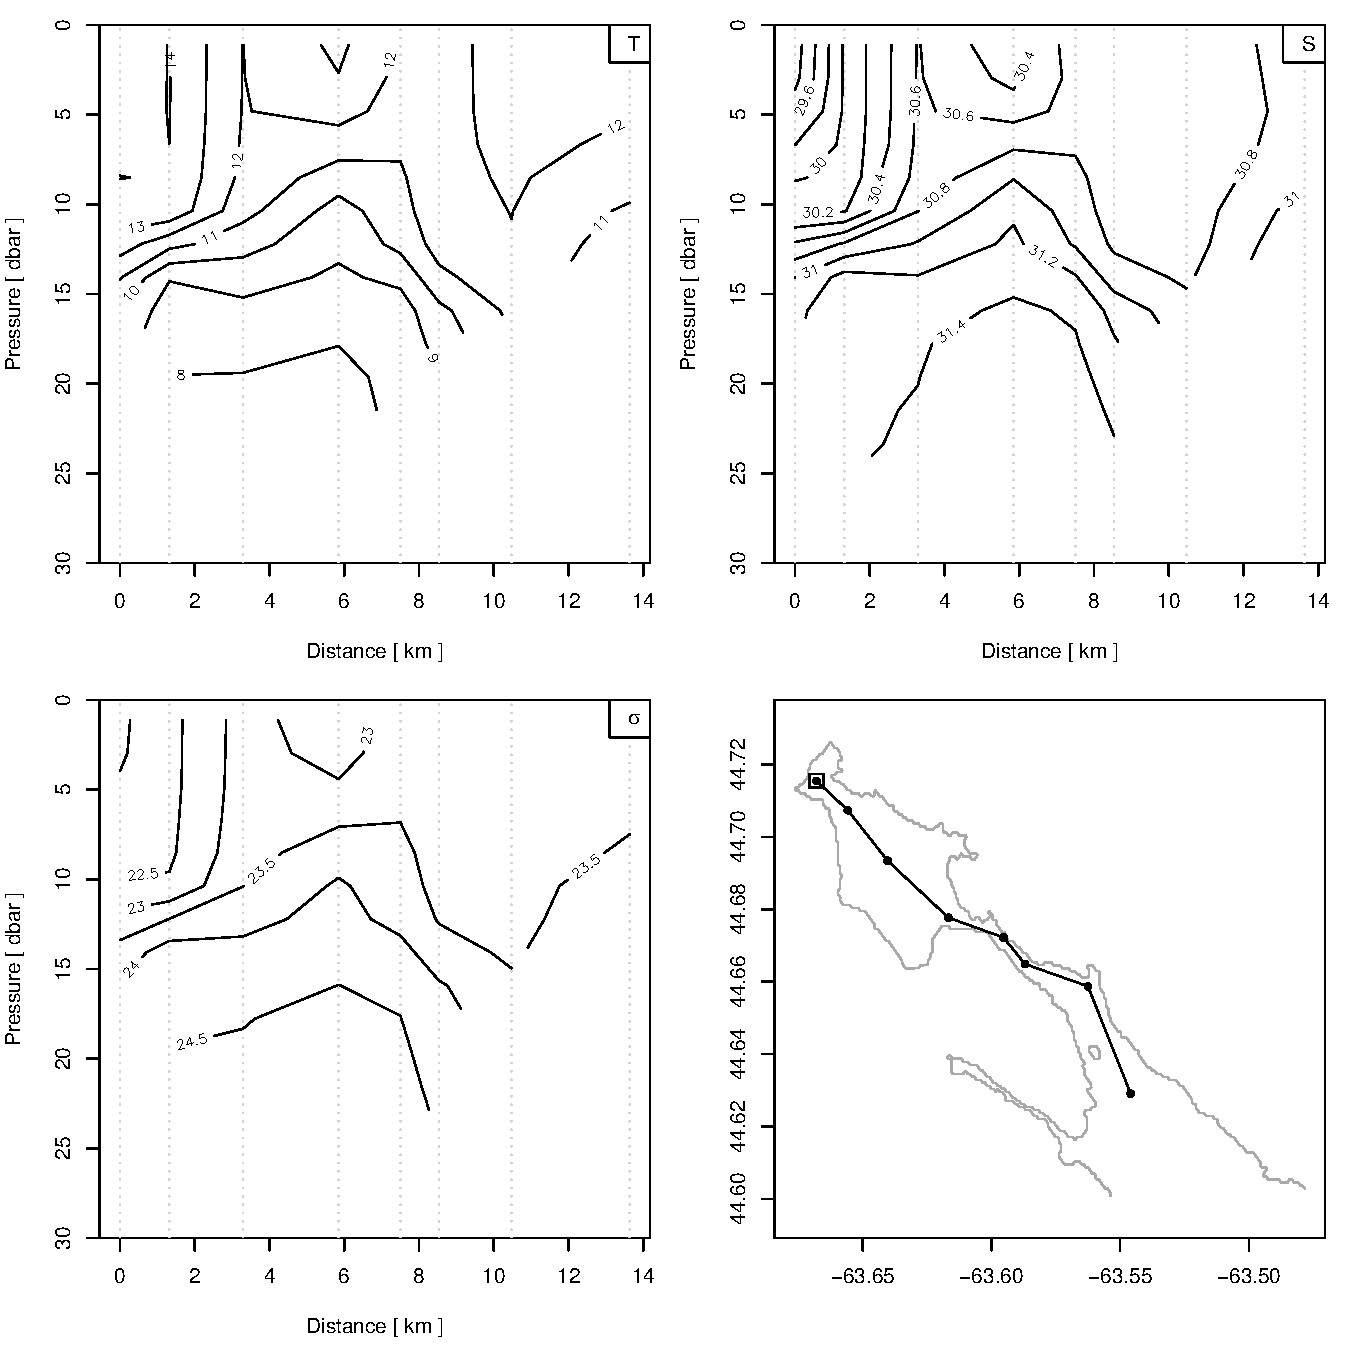
\includegraphics{oce-sectionfig}
\end{center}
\caption{\label{fig:section}
CTD section of data acquired in Halifax Harbour in the autumn of 2003 by
students in the \emph{Introduction to Physical Oceanography} class at Dalhousie
University.  (Dan Kelley teaches this class, and the work at sea was supervised
by his teaching assistant Natacha Bernier, who received her PhD from Dalhousie
in 2005.)  The stations go from a site near the Sackville river inflow at the
northwest portion of Bedford Basin to site at the entrance of the harbour. (The
author's office at Dalhousie is located near the bottom axis at 63.58W.)}
\end{figure}

\index{reading!ctd section}
\index{data!section \verb@a03@, North Atlantic along 36$^\circ$N}

\index{Gulf Stream}

The Halifax section is supplied in a pre-gridded format, but some datasets have
different pressure levels at each station.  For such cases, the
\verb@section.grid@ function may be used, e.g.
\begin{Schunk}
\begin{Sinput}
> data(a03)
> Gulf.Stream <- section.subset(a03, 124:102)
> Gulf.Stream.gridded <- section.grid(Gulf.Stream, p = seq(0, 5000, 
+     10))
> data(coastline.world)
> plot(Gulf.Stream.gridded, coastline = coastline.world, map.xlim = c(-80, 
+     -60))
\end{Sinput}
\end{Schunk}
produces Figure~\ref{fig:sectiona03}.  The ship doing the sampling was
travelling westward from the Mediterranean towards North America, taking 124
stations in total; the \verb@station.indices@ value selects the last few
stations of the section, during which the ship heading was changed to run in a
northwesterly direction, to cross isobaths (and perhaps, the Gulf Stream) at
right angles.

\begin{figure}
\begin{center}
\setkeys{Gin}{width=1\textwidth}
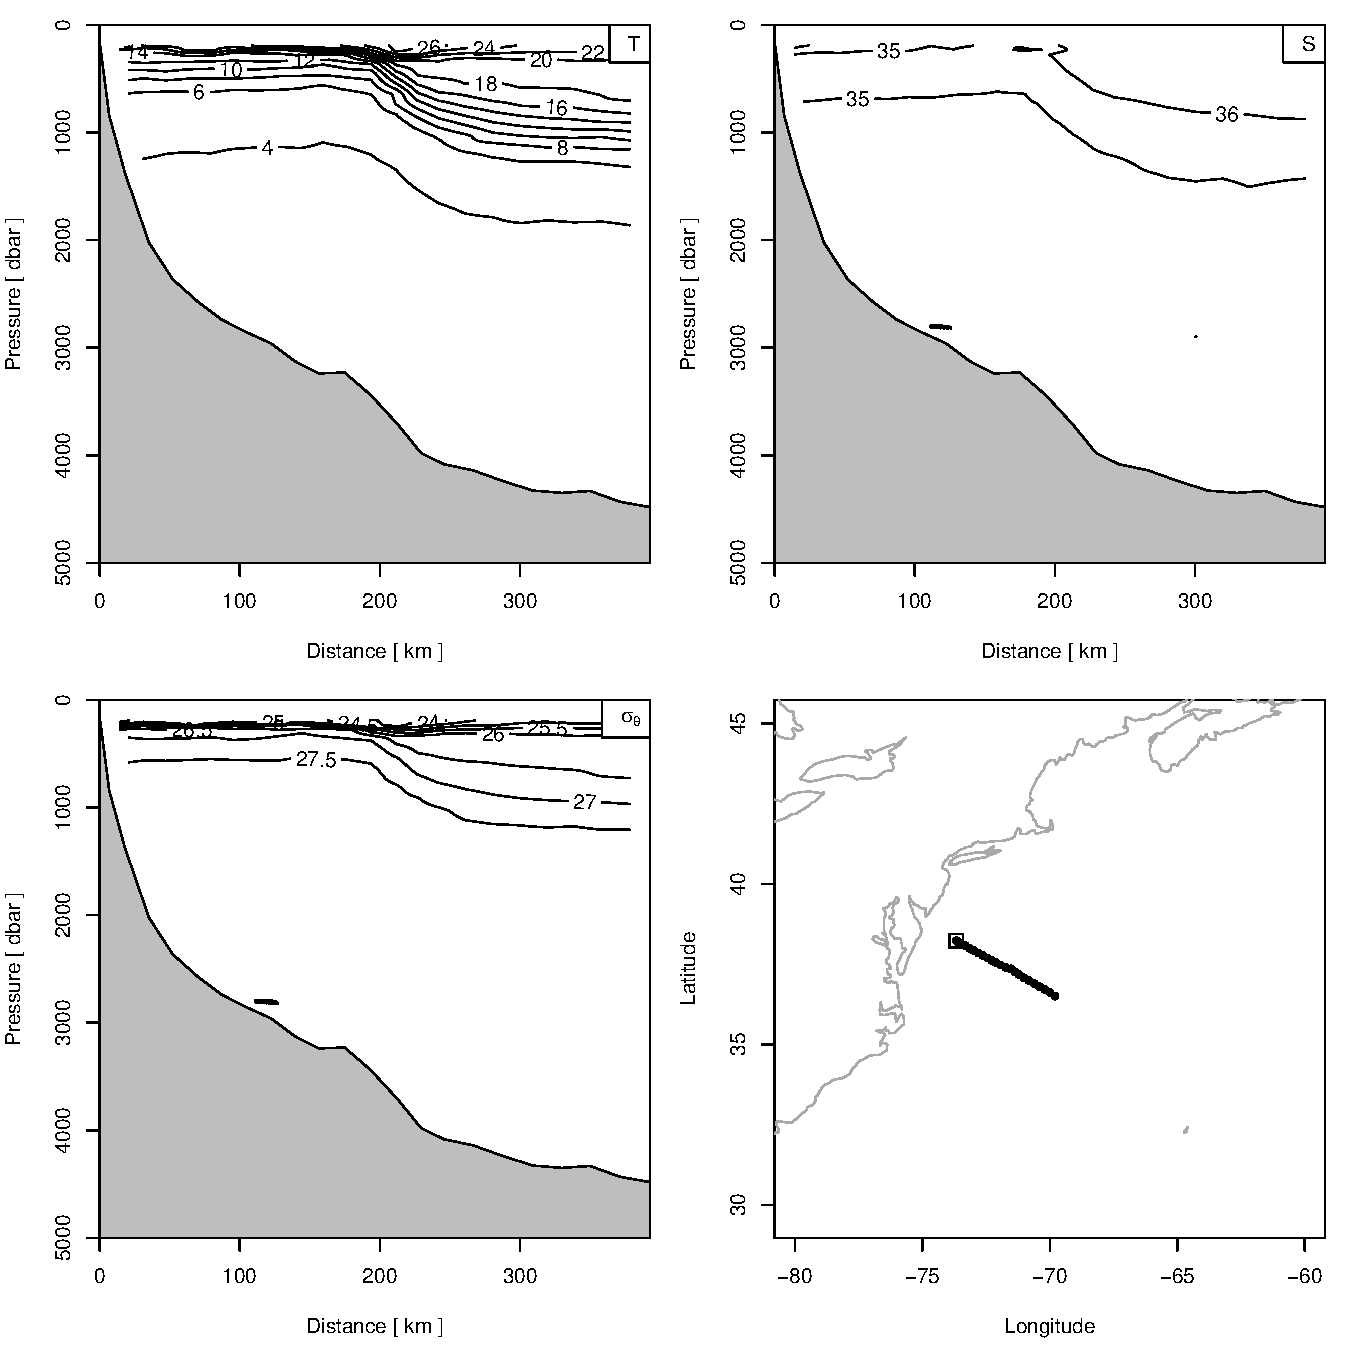
\includegraphics{oce-sectionfiga03}
\end{center}
\caption{\label{fig:sectiona03}
Portion of the CTD section designated A03 (Cruise chief scientist: Tereschenkov, SOI.), showing the region of the Gulf Stream.  (The small number of S contours
in the upper water column is the result of a near-bottom salinity anomaly
in the station at about 200km.)
}
\end{figure}

\workedexercise{4}{Plot dynamic height across the Gulf Stream, and show the corresponding geostrophic velocity.}

\section{Coastline data}

\index{data!coastline}

The commands
\begin{Schunk}
\begin{Sinput}
> library(oce)
> data(coastline.maritimes)
> plot(coastline.maritimes, col = "darkred")
> points(-(63 + 34/60), 44 + 39/60, cex = 3, col = "blue")
\end{Sinput}
\end{Schunk}
produce a map of the coastline of Eastern Canada
(Figure~\ref{fig:coastline}). Such coastline data are available from a variety
of sources. The NOAA site \url{http://www.ngdc.noaa.gov/mgg_coastline/} is
particularly popular, and it has the advantage of providing data in Splus
format.  The function \verb@read.coastline@ can handle reading that format (plus
some other formats).
\begin{figure}
\begin{center}
\setkeys{Gin}{width=0.5\textwidth}
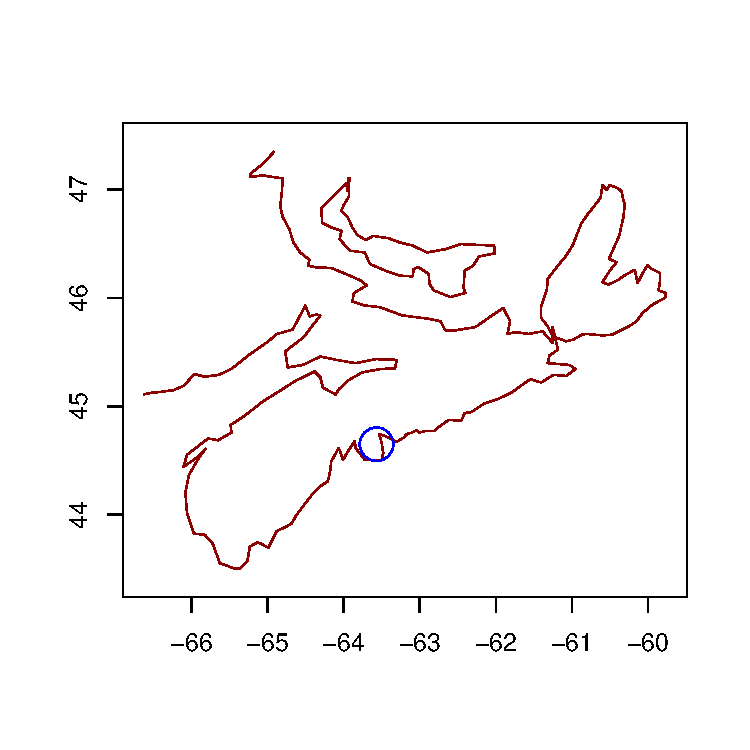
\includegraphics{oce-coastlinefig}
\end{center}
\caption{Coastline of eastern Canada, showing Prince Edward Island, New
Brunswick, and Nova Scotia.  The blue circle indicates the location of Halifax,
the capital of Nova Scotia.}
\label{fig:coastline}
\end{figure}

\section{Sea-level data}

\subsection{Time-domain analysis}

\index{sea level!during Hurricane Juan}
\index{Hurricane Juan!surge seen in time-series of sea level}

The commands
\begin{Schunk}
\begin{Sinput}
> library(oce)
> data(sealevel.hal)
> plot(sealevel.hal)
\end{Sinput}
\end{Schunk}
load and graph a build-in dataset of sea-level timeseries. The result, shown in
Figure~\ref{fig:sealevel}, is a four-panel plot. The top panel is a timeseries
view that provides an overview of the entire data set. The second panel is
narrowed to the most recent month, which should reveal spring-neap cycles if the
tide is mixed. The third panel is a spectrum, with a few tidal constituents
indicated. At the bottom is a cumulative spectrum, which makes these
narrow-banded constituents quite visible.

\begin{figure}
\begin{center}
\setkeys{Gin}{width=.8\textwidth}
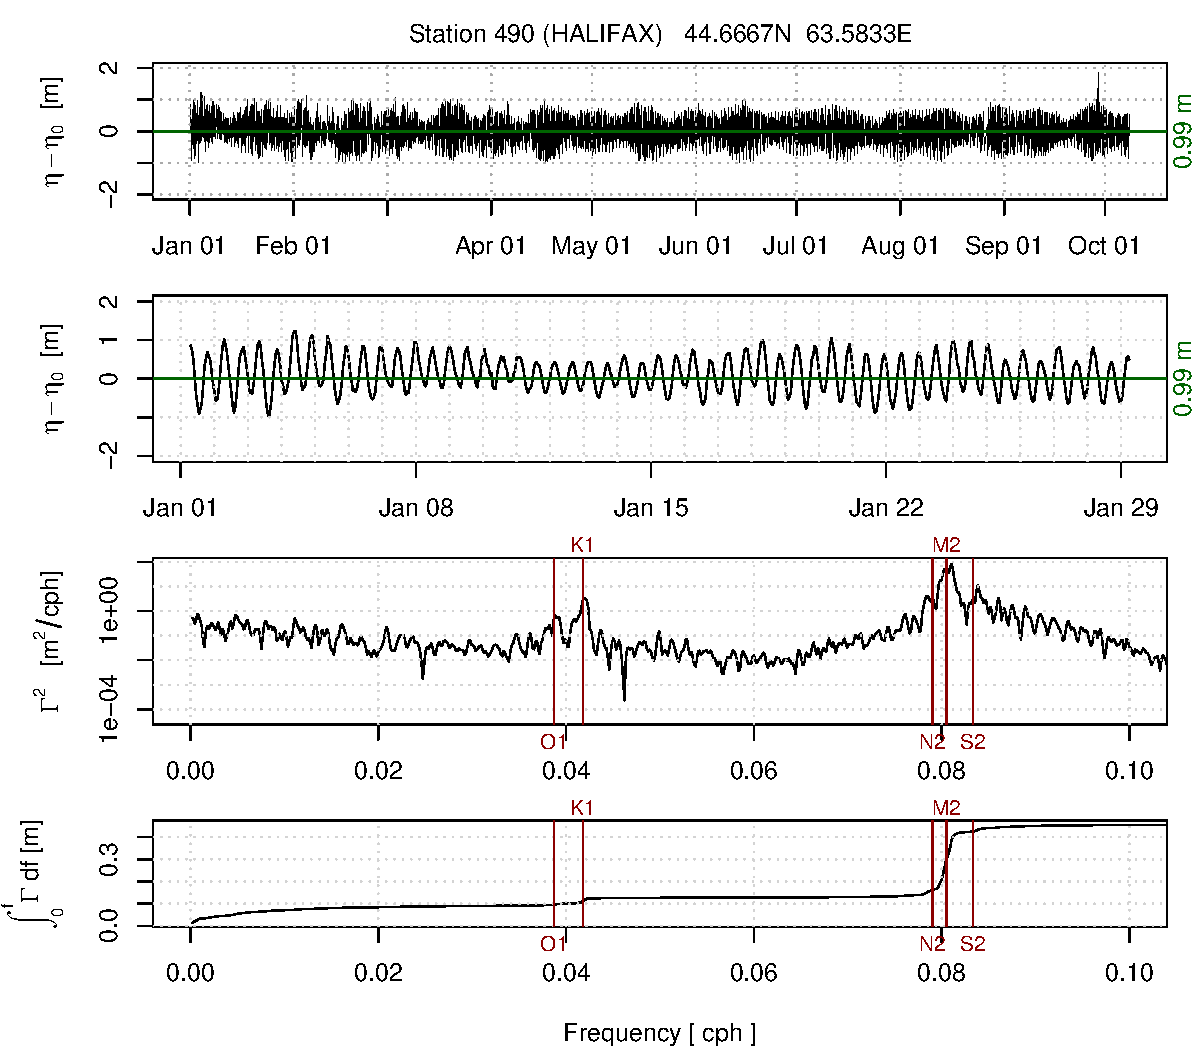
\includegraphics{oce-sealevelfig}
\end{center}
\caption{Sea-level timeseries measured in 2003 in Halifax Harbour.  (The spike
in September is the storm surge associated with Hurricane Juan, regarded by the
Canadian Hurricane Centre to be one of the most powerful and damaging hurricanes
to ever hit Canada.}
\label{fig:sealevel}
\end{figure}

\workedexercise{5}{Illustrate Halifax sealevel variations during Hurricane Juan}

\workedexercise{6}{Draw a spectrum of sea-level variation, with the M2 tidal component indicated.}

\subsection{Tidal analysis}

Tidal analysis is provided in a rudimentary way, as is illustrated in the
example below, which shows the storm surge experienced in Halifax in 2003, with
Hurricane Juan.

\index{sea level!storm surge during Hurricane Juan}
\index{Hurricane Juan!surge detection by detiding}

\begin{Schunk}
\begin{Sinput}
> library(oce)
> data(sealevel.hal)
> tide <- tidem(sealevel.hal)
> days <- 15
> n <- length(sealevel.hal$data$eta)
> i <- seq(n - 24 * days, n)
> t <- sealevel.hal$data$t[i]
> eta <- sealevel.hal$data$eta[i]
> eta.pred <- predict(tide)[i]
> plot(t, eta, type = "l", ylim = c(-0.5, 3))
> abline(h = 0, col = "pink")
> lines(t, eta - eta.pred, col = "red")
\end{Sinput}
\end{Schunk}
produce Figure~\ref{fig:tide}, illustrating the use of tidal analysis to detect
storm surges.  Note the use of the \verb@model@ that is returned by the tide
analysis.

(It should be noted that the tidal analysis portion of \verb@oce@ is still in
active development, and the features are subject to change.  Use
\verb@?tidem@ to learn more about this.)

\begin{figure}
	\begin{center}
\setkeys{Gin}{width=0.8\textwidth}
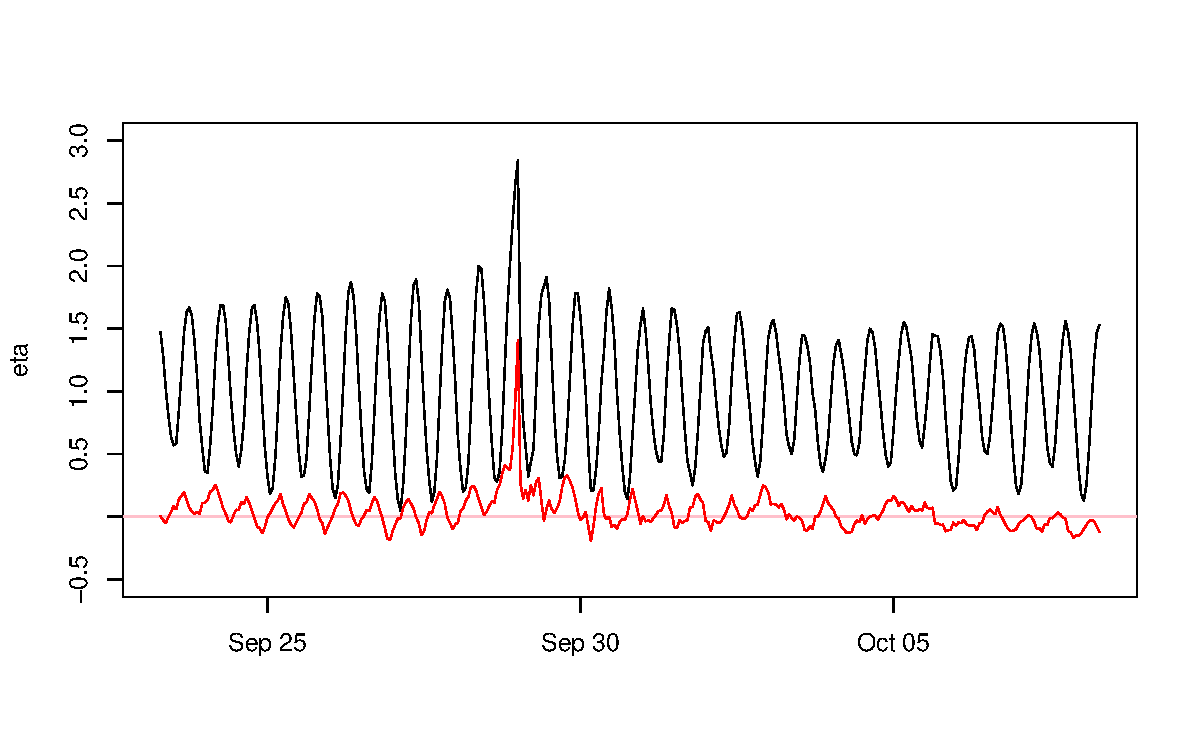
\includegraphics{oce-tidefig}
\end{center}
\caption{Sea-level variation in Halifax Harbour in 2003 (black line) and the residual
after removal of tides using \texttt{tidem()}.  The spike on September 28th
is a storm surge caused by Hurricane Juan, which caused a great deal of damage
to the region.}
\label{fig:tide}
\end{figure}

\goodbreak


\section{Lobo data}
The commands
\begin{Schunk}
\begin{Sinput}
> library(oce)
> data(lobo)
> plot(lobo)
\end{Sinput}
\end{Schunk}
produce a plot (Figure~\ref{fig:lobo}) of lobo data from the Northwest Arm of
Halifax Harbour.  Note the relationship between decreasing nutrients and
increasing fluorescence, as well as the diurnal signal in the latter.

The reader should note that the \verb@lobo@ part of \verb@oce@ is somewhat
preliminary. In particular, the package requires that certain data columns be
present, and in a certain order. Also, the function \verb@read.oce@ does not
understand \verb@lobo@ files. Why these limitations, you ask? Well, the
\verb@lobo@ code was really only written as an aside, for the author's
contribution to a ``predict the spring bloom'' contest held at Dalhousie
University.

\begin{figure}
\begin{center}
\setkeys{Gin}{width=0.66\textwidth}
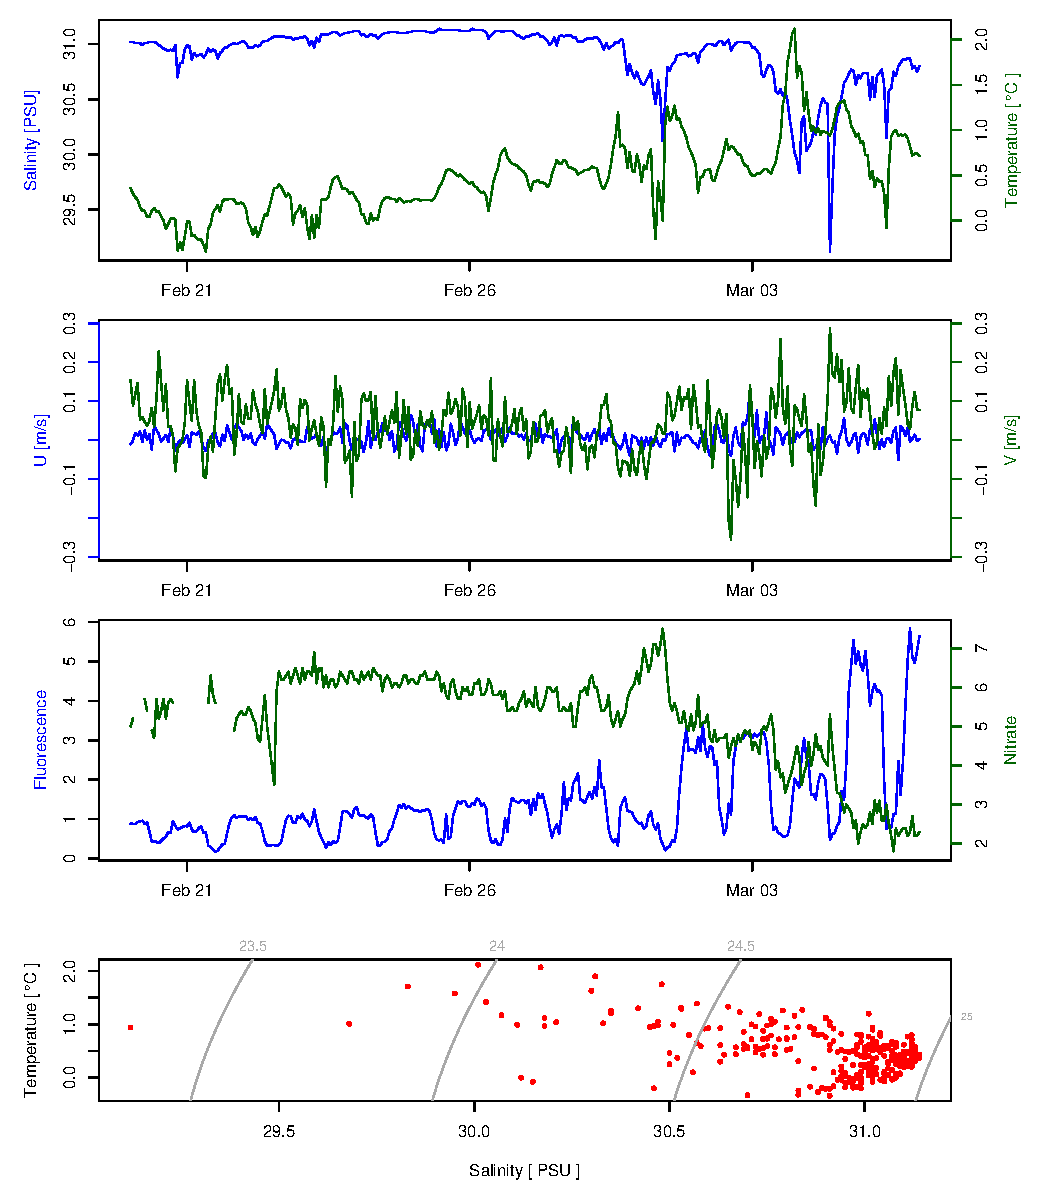
\includegraphics{oce-lobofig}
\end{center}
\caption{Lobo measurements in Northwest Arm of Halifax Harbour, at
the time of the 2007 Spring bloom.}
\label{fig:lobo}
\end{figure}

\workedexercise{7}{Draw a $T-S$ plot for these data, using a colour coding to indicate time,
and using plotting tricks to reduce the obscuring of this time signal.}


\section{The future of oce}

The present version of \verb@oce@ can only handle data types that the author has
been using lately in his research. New data types will be added as the need
arises in that work, but the author would also be happy to add other data types
that are likely to prove useful to the Oceanographic community.  (The data types
need not be restricted to Physical Oceanography, but the author will need some
help in dealing with other types of data, given his research focus.)

As for algorithms, there are plenty of gaps in \verb@oce@.  Dealing with
measurements of turbulence is a high priority for the author, for example, and
it is also clear that there are some methods of ADP processing that should be
provided by the package.

Two principles will guide the addition of data types and functions:
(a) the need, as perceived by the author or by other contributors and
(b) the ease with which the additions can be made.

The site \url{http://code.google.com/p/r-oce/} provides a window on the
development that goes on between the CRAN releases of the package. Please visit
the site to report bugs, to suggest new features, or just to see how \verb@oce@
development is coming along.

%\begin{center}
%\vspace{2cm}
%
%------
%
%\vspace{2cm}
%
%See the end of the document for answers to exercises.
%
%\end{center}
%
%\newpage

\goodbreak

\section*{Answers to exercises}

\workedanswer{1}{Seawater properties}
\begin{Schunk}
\begin{Sinput}
> library(oce)
> sw.rho(S = 34, t = 10, p = 100)
\end{Sinput}
\begin{Soutput}
[1] 1026.624
\end{Soutput}
\begin{Sinput}
> sw.theta(S = 34, t = 10, p = 100)
\end{Sinput}
\begin{Soutput}
[1] 9.988598
\end{Soutput}
\begin{Sinput}
> sw.rho(S = 34, t = sw.theta(S = 34, t = 10, p = 100), p = 0)
\end{Sinput}
\begin{Soutput}
[1] 1026.173
\end{Soutput}
\begin{Sinput}
> sw.rho(S = 34, t = sw.theta(S = 34, t = 10, p = 100, pref = 200), 
+     p = 200)
\end{Sinput}
\begin{Soutput}
[1] 1027.074
\end{Soutput}
\begin{Sinput}
> plot.TS(as.ctd(c(30, 40), c(-2, 20), rep(0, 2)), grid = TRUE, 
+     col = "white")
\end{Sinput}
\end{Schunk}

\workedanswer{2}{Profile plots}
Although one may argue as to the limits of the pycnocline, for illustration let us say it is in 5bar to 12dbar range.
\begin{Schunk}
\begin{Sinput}
> library(oce)
> data(ctd)
> pycnocline <- ctd.trim(ctd, "pressure", c(5, 12))
> plot.profile(pycnocline, type = "density+N2")
\end{Sinput}
\end{Schunk}

\index{section!extracting profile data from}
\workedanswer{3}{TS diagram for section data}
\begin{Schunk}
\begin{Sinput}
> library(oce)
> data(section)
> SS <- TT <- pp <- id <- NULL
> n <- length(section$data$station)
> for (i in 1:n) {
+     stn <- section$data$station[[i]]
+     SS <- c(SS, stn$data$salinity)
+     TT <- c(TT, stn$data$temperature)
+     pp <- c(pp, stn$data$pressure)
+     id <- c(id, rep(i, length(stn$data$pressure)))
+ }
> ctd <- as.ctd(SS, TT, pp)
> plot.TS(ctd, col = hsv(0.7 * id/n), cex = 2, pch = 21)
\end{Sinput}
\end{Schunk}

\workedanswer{4}{Gulf Stream}
(Try \verb@?sw.dynamic.height@ for hints on smoothing.)
\index{Gulf Stream!geostrophic calculation}
\begin{Schunk}
\begin{Sinput}
> library(oce)
> data(a03)
> Gulf.Stream <- section.subset(a03, 124:102)
> dh <- sw.dynamic.height(Gulf.Stream)
> par(mfrow = c(2, 1))
> plot(dh$distance, dh$height, type = "b", xlab = "", ylab = "Dyn. Height [m]")
> grid()
> f <- coriolis(Gulf.Stream$data$station[[1]]$metadata$latitude)
> g <- gravity(Gulf.Stream$data$station[[1]]$metadata$latitude)
> v <- diff(dh$height)/diff(dh$distance) * g/f/1000
> plot(dh$distance[-1], v, type = "l", col = "blue", xlab = "Distance [km]", 
+     ylab = "Velocity [m/s]")
> grid()
> abline(h = 0)
\end{Sinput}
\end{Schunk}
\workedanswer{5}{Halifax sealevel during Hurricane Juan}
\index{Hurricane Juan!worked example of sea-level plot}
\index{sea level!during Hurricane Juan}
A web search will tell you that Hurricane Juan hit about midnight, 2003-sep-28.
The author can verify that the strongest winds occurred a bit after midnight -- that was the time
he moved to a room without windows, in fear of flying glass.
\begin{Schunk}
\begin{Sinput}
> library(oce)
> data(sealevel.hal)
> plot(sealevel.hal, focus.time = c("2003-09-23", "2003-10-05"))
> abline(v = as.POSIXct("2003-09-28 23:30:00"), col = "red", lty = "dotted")
> mtext("Hurricane\nJuan", at = as.POSIXct("2003-09-28 23:30:00"), 
+     col = "red")
\end{Sinput}
\end{Schunk}

\workedanswer{6}{Sealevel spectrum}
Notice the use of \verb@(object)$data$(item)@ here.  All \verb@oce@ objects are lists,
and all of them contain a \verb@data@ element of a similar form to this.
\begin{Schunk}
\begin{Sinput}
> library(oce)
> data(sealevel.hal)
> spectrum(sealevel.hal$data$eta, spans = c(3, 7))
> abline(v = 1/12.42)
> mtext("M2", at = 1/12.42, side = 3)
\end{Sinput}
\end{Schunk}

\workedanswer{7}{Lobo plot}
\index{data!lobo timeseries}
The resampling with \verb@i@ is to avoid obscuring colours by overplotting.
Note the use of \verb@as.ctd@ to assemble the data into something that
\verb@plot.TS@ can handle.  This is an example of the practicality of
\verb@oce@; eventually, \verb@plot.TS@ may be altered to take simple columns of
data, but for now it seems reasonable to require the user to assemble these data
into a CTD object, and to spend development time on something that will pay off
better.
\begin{Schunk}
\begin{Sinput}
> library(oce)
> data(lobo)
> i <- sample(length(lobo$data$temperature))
> a <- as.numeric(lobo$data$time[i] - lobo$data$time[1])
> col <- hsv(0.5 * a/max(a), 1, 1)
> plot.TS(as.ctd(lobo$data$salinity[i], lobo$data$temperature[i], 
+     0), col = col, pch = 1)
\end{Sinput}
\end{Schunk}


\printindex
\end{document}
